\documentclass[pdftex,12pt,a4paper]{report}

\usepackage[dvipsnames]{xcolor}
\usepackage[pdftex]{graphicx}
\usepackage{float}
\usepackage{fancyvrb}
\usepackage{dtklogos}
\fvset{xleftmargin=2em}

\usepackage{pgfplots}
\pgfplotsset{width=10cm,compat=1.9}
\usepackage{tikzscale}
\usepackage{pgfplotstable}
\usepackage{booktabs}
\usepackage[font=small,labelfont=bf,tableposition=top]{caption}

\usepackage[utf8]{inputenc}
\usepackage[portuges]{babel}
\usepackage[T1]{fontenc}
\usepackage{times}
%\usepackage{lmodern}
\usepackage[obeyspaces,spaces]{url}
\usepackage[left=20mm,right=20mm,top=25mm,bottom=25mm]{geometry}
\usepackage{titlesec}
\usepackage{mathtools}
\usepackage{amsfonts}

%identa 1º paragrafo de capitulos e secções
\usepackage{indentfirst}
\usepackage{url}
%\usepackage{alltt}
\usepackage[]{hyperref}
\usepackage{xspace}

\hypersetup{
%pdftitle={Trabalho 1 - Gestão de Projeto},
%pdfauthor={Bruno Pereira},
%pdfsubject={Investigação Operacional},
%pdfkeywords={keyword1, keyword2}},
bookmarksnumbered=true,     
bookmarksopen=true,         
bookmarksopenlevel=1,       
colorlinks=true,            
pdfstartview=Fit,           
pdfpagemode=UseOutlines, % this is the option you were lookin for
pdfpagelayout=TwoPageRight
		}

\usepackage{minted}
\usemintedstyle{borland}
\setminted{
%frame=lines,
%framesep=2mm,
baselinestretch=1.2,
fontsize=\footnotesize,
%linenos, 
%breaklines,
%breakautoindent=false,
autogobble
}
\usepackage{caption}

\def\BibTeX{{\rm B\kern-.05em{\sc i\kern-.025em b}\kern-.08em
    T\kern-.1667em\lower.7ex\hbox{E}\kern-.125emX}}

\newenvironment{longlisting}{\captionsetup{type=listing}}{}
\def\darius{\textsf{Darius}\xspace}

\def\java{\texttt{Java}\xspace}

\def\pe{\emph{Publicação Eletrónica}\xspace}

\newcommand{\HRule}{\rule{\linewidth}{0.5mm}}


\begin{document}

\begin{titlepage}


\begin{minipage}{0.3\textwidth}
\begin{flushleft} 

\includegraphics[width=1.1\textwidth]{./report/logo.png}
\end{flushleft}
\end{minipage}
\hfill
\begin{minipage}{0.6\textwidth}
\begin{flushright} 

\fontfamily{pag}\selectfont{\large \textsc{Departamento de Informática}\\[0.1cm]
\large \bfseries Mestrado Integrado em Engenharia Informática \\ [0.1cm]
\large \bfseries \textit{Processamento de Linguagens}\\[4mm]
}
\noindent\rule{\textwidth}{0.7mm}
\end{flushright}
\end{minipage}\\[1cm]


\vspace{3cm}


\begin{center}

\fontfamily{pag}\selectfont{\textsc{\Huge Trabalho Prático nº 1}\\[1cm]


{\large \bfseries \emph{Normalizador de ficheiros \hologo{BibTeX}} \\[2cm] }

\vfill
\begin{minipage}{0.4\textwidth}
	\begin{flushleft} 
		\large
	Bruno Pereira\\
\textbf{Aluno nº 72628} 
	\end{flushleft}

\end{minipage}
\begin{minipage}{0.4\textwidth}
	\begin{flushright} 
		\large
	Ricardo Oliveira\\
\textbf{Aluno nº 58657} 
	\end{flushright}
\end{minipage}

\vfill



\vfill

\emph{\large Braga, {\large \today}}
}
\end{center}

\end{titlepage}

\begin{abstract}
Isto é um resumo do relatório de \pe focando o contexto do trb (muito
sucinto),os objetivos concretos e os resultados atingidos.

Algum texto curto mas que entusiasme a leitura do relatório de \pe.

\end{abstract}

\tableofcontents

\chapter*{Introdução}
\addcontentsline{toc}{chapter}{Introdução} 
\label{intro}


O presente documento visa a documentação do processo de aprendizagem de
especificações em \emph{Flex} e criação de filtros para diversos formatos de
texto. No contexto escolhido, criações de filtros para ficheiros
\hologo{BibTeX}. Numa primeira parte, o objetivo é a criação de uma filtro para
contabilizar as entradas bibliográficas e criar um ficheiro \emph{HTML} com
o resultado. Ficheiros deste género podem crescer muito em tamanho, por vezes
uma contabilização pode ajudar a construir repositórios documentais sobre
determinado assunto. De igual modo, a necessidade de normalização de um
documento deste é importante, porque com o passar do tempo, o acrescentar novas
entradas pode criar desvios de formatação, que pode prejudicar uma pesquisa no
documento pelo nome, por exemplo. Um exemplo de um normalizador deste género
figura na segunda parte (capítulo 2) deste documento.  Além do normalizador, na
terceira parte (cap. 3), é apresentado a elaboração de um filtro para fazer um
\emph{pretty-printing} de um documento \hologo{BibTeX}.  Por último, no quarto
capítulo é apresentada uma ferramenta para criar um grafo com os coautores de
determinado autor, onde os pesos das arestas são a densidade de publicação com
cada coautor.


\section*{Metas e objetivos} 

O ambiente Linux é uma das metas deste trabalho. Existem diversas formas de
fazer determinadas coisas para fazer em Linux, onde cada ferramenta tem o seu
lugar e não faltam ferramentas.  O domínio deste sistema operativo é importante,
dado que, um programador, com conhecimento suficiente sobre este sistema
operativo, tem uma liberdade que falta a outros. De igual modo, dado que as
ações das especificações no \emph{Flex} são programadas em linguagem C, um dos
objetivos passa por refinar e aumentar o conhecimento da linguagem, bem como
aprofundar o conhecimento em estruturas mais complexas. De igual modo,
algoritmos e complexidade são serão revisitados, e a otimização será algo
importante durante a elaboração do trabalho. Pretende-se, portanto, soluções
eficientes. Por último, o grande objetivo é desenvolver a capacidade de escrita
de \emph{ER's} e entender como o funcionamento de processadores de linguagens
regulares funcionam, usando geradores de filtros de texto como o \emph{Flex}.
Deste último objetivo será testemunha este documento.  


\section*{Estrutura do Relatório} 
O relatório está organizado em 4 capítulos: o primeiro capítulo é referente
à alínea \emph{a}, o segundo e terceiros capítulos correspondem à alínea
\emph{b} e o quarto capitulo corresponde à alínea \emph{c}.  Cada capítulo
possui três secções: \emph{Análise do Problema}, \emph{Desenho e implementação
da solução} e \emph{Testes e Resultados}.  Na secção \emph{Análise do Problema}
expõe-se informalmente o problema, contendo conteúdo referentes aos dados,
relações e possíveis abordagens à solução. Na secção \emph{Desenho
e implementação da solução} descrevem-se as especificações e respetivas ações do
\emph{Flex}, \emph{START CONDITION}, estruturas de dados e algoritmos e funções
importantes. Em seguida a secção \emph{Testes e Resultados} apresenta os
resultados e acrescenta uma breve discussão sobre problemas de implementação,
alternativas e sugestões.  Note-se que neste documento, para mostrar
a extensibilidade dos testes, muitos deles estão no \emph{Apêndice}. O documento
encerra com a \emph{Conclusão} onde se avaliará a completude dos objetivos, bem
como observações aos resultados obtidos.






\chapter{Contagens de categorias de um ficheiro \hologo{BibTeX}}
\label{chap:a}

\section{Análise do Problema}
Neste primeiro problema, pretende-se analisar um documento \hologo{BibTeX} e fazer as
contagens das respetivas categorias, tais como artigos, teses de mestrado,
manuais, etc. O resultado tem que constar num ficheiro \texttt{HTML}.


\label{sec:ap:a}

\subsection{Especificação dos requisitos}
\label{sec:spec:a}
Existem pelo menos 14 tipos de entradas bibliográficas no \hologo{BibTeX},
podendo haver algumas extensões ou pacotes que possuam outras --- como por exemplo
o \textsc{Bib}\LaTeX{}.
Note-se que, a distinção entre o formato de ficheiro \hologo{BibTeX}
e o programa \hologo{BibTeX} é importante. O pacote \textsc{Bib}\LaTeX{} pode
ser usado tanto pelo programa \hologo{BibTeX} como não, uma vez que
o \emph{backend} por defeito do \textsc{Bib}\LaTeX{} --- o \emph{biber} ---
suporta o formato de ficheiro \hologo{BibTeX} (\texttt{.bib}). Assim, os
utilizadores do \textsc{Bib}\LaTeX{} podem usar o mesmo ficheiro \texttt{.bib} com
poucas alterações. Em consequência pode-se afirmar, que em cada ficheiro
\texttt{.bib}, todos os tipos de entrada começam com \emph{\@}, ora usam
o \hologo{BibTeX}, ora usem o \textsc{Bib}\LaTeX.


\subsection{Dados}

Os 14 tipos de entradas bibliográficas do \hologo{BibTeX} são:

\begin{itemize}
	\item\textbf{Article      } Um artigo de um jornal ou revista.
    
	\item\textbf{Booklet      } Um livro não publicado por uma editora, mas que
		é impresso e encadernado.
       
	\item\textbf{Book         } Um livro publicado por uma editora.
       
	\item\textbf{Conference   } O mesmo que \emph{Inproceedings}. 
	\item\textbf{Inbook       } Uma parte de um livro, o qual pode ser um capítulo (ou secção ou outro qualquer) e/ou uma série de páginas.
      
	\item\textbf{Incollection } Uma parte de um livro que tem o seu próprio título.
     
	\item\textbf{Inproceedings} Um artigo de uma coleção de \emph{papers} académicos de uma conferência.
   
	\item\textbf{Manual       } Documentação técnica. 
  
	\item\textbf{Mastersthesis} Uma tese de mestrado.
	\item\textbf{Misc         } Qualquer outro documento que não se enquadre em nenhuma
		catgoria.
       
	\item\textbf{Phdthesis    } Uma tese de doutoramento.
      
	\item\textbf{Proceedings  } Coleção de \emph{papers} académicos de uma conferência.
     
	\item\textbf{Techreport   } Um relatório publicado por uma escola ou outra instituição.
    
	\item\textbf{Unpublished  }  Um documento com um autor e título, mas não formalmente
		publicado.

\end{itemize}

Para além destes tipo de entradas existem também as entradas \texttt{@STRING},
\texttt{@PREAMBLE} e \texttt{@COMMENT}, onde a primeira serve para definir
abreviaturas para serem usadas no ficheiro \hologo{BibTeX}, a segundá define
como texto especial deve ser formatado, e a última, serve para incluir
comentários que não devem ser tidos em conta pelo \hologo{BibTeX}.



\section{Desenho e implementação da solução}
\label{sec:des:a}

\subsection{Expressões Regulares}
Antes de se iniciar a descrição, note-se que as \emph{ERs} estão ordenadas de
forma a não haver ambiguidade.


Uma entrada de um ficheiro \hologo{BibTeX} começa sempre com \texttt{@}. De
igual modo, os nomes de tipos de entrada podem ser escritos com maiúsculas ou
minúsculas, bem como podem começar por uma maiúscula, seguidas de minúsculas. Em
suma, não é \emph{case sensitive}. Assim, na especificação do \emph{Flex},
podemos definir uma entrada como um conjunto de caracteres, que começa com
\texttt{@} seguido de uma ou mais ocorrências de caracteres, maiúsculos ou
minúsculos.

Todavia, é necessário especializar a especificação, relativamente às entradas
\texttt{@STRING}, \texttt{@PREAMBLE} e \texttt{@COMMENT}. Também, para os tipos
de entrada bibliográficos é necessário especializar a expressão regular para os
tipos comuns de entradas descritos na secção anterior. A razão desta última
especialização justifica-se apenas por motivos de otimização e eficiência do
filtro, que serão respondidos nas secções seguintes. 

Desta forma temos 4 \emph{ER's}:

\begin{itemize}
	\item Uma expressão regular para capturar ou \texttt{@STRING},
		\texttt{@PREAMBLE} e \texttt{@COMMENT}, da seguinte forma:
\begin{minted}{text}
		\@[Ss][Tt][Rr][Ii][Nn][Gg]
		\@[Pp][Rr][Ee][Aa][Mm][Bb][Ll][Ee]
		\@[Cc][Oo][Mm][Mm][Ee][Nn][Tt]
\end{minted}

A ação nestas expressões regulares é para ignorar.


	\item Uma expressão regular para capturar uma entrada específica, por exemplo:
		\mint{text}|\@[Aa][Rr][Tt][Ii][Cc][Ll][Ee]| para capturar uma ocorrência de
		\texttt{ARTICLE}.

		A ação é contabilizar a ocorrência. Para a contabilização de \emph{ER's}
		deste género, usou-se uma vetor de inteiros, de tamanho 14, em que cada
		posição corresponde a um tipo de entrada.
\newpage

	\item Uma expressão regular para capturar uma entrada genérica, por exemplo:
		\mint{text}|\@[A-Za-z]+| onde o valor capturado é copiado a partir do
		caractere \texttt{@} e inserido numa tabela de
		\emph{hash}, contabilizando repetições.Especificações da tabela de
			\emph{hash} encontram-se na secção seguinte.
	\item Uma expressão regular para ignorar tudo o resto.

\end{itemize}


Por fim, existe a nuance de se fazer a travessia da
tabela de \emph{hash} se houver elementos na tabela.


\subsection{Estruturas de dados}
\label{sec:subsec:es:a}
Escolheu-se uma tabela de \emph{hash} dinâmica que usa o método de
\emph{chaining},
a \texttt{uthash}\footnote{\url{https://troydhanson.github.io/uthash/}} para
utilização neste problema.  Esta possui uma complexidade em termos de tempo
constante na adição, remoção e procura, bem como tem uma melhor gestão de
memória. No entanto, embora haja tabelas mais rápidas, utilizou-se esta tabela
por uma questão de conveniência, dada a simplicidade e ter \emph{performance}
aceitável para este problema.\footnote{\emph{Benchmarking} relativamente
a outras estruturas pode ser encontrado em
\url{http://lh3lh3.users.sourceforge.net/udb.shtml.}}


\section{Testes e Resultados}
\label{sec:ts:a}


\subsection{Resultados}
Para testar o filtro, utilizou-se o ficheiro \hologo{BibTeX} dado como exemplo
em \url{http://www4.di.uminho.pt/~prh/lp.bib}.

O resultado em \emph{HTML} consta no Apêndice~\ref{appendix:a}, na
pág.~\pageref{appendix:a}.

O resultado após ser executado por um \emph{browser} é o que se segue:

\begin{figure}[h!]
	\centering
	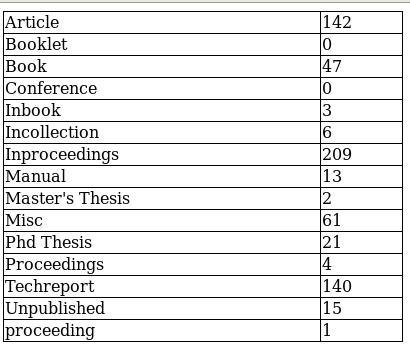
\includegraphics[scale=0.5]{./testes/res_html}
	\caption{Resultado visto no \emph{Firefox}}
	\label{fig:res1}
\end{figure}

A partir do documento que adveio da URL na secção \emph{Resultados}, podemos
constar que não existem entradas que difiram do \hologo{BibTeX}, a não ser
a entrada \emph{proceeding}, e que não existem \emph{Booklets}, nem
\emph{Conferences}. 


\subsection{Alternativas, Decisões e Problemas de Implementação}

Numa primeira implementação, existia uma \emph{trie} para guardar os tipos de
entrada que não pertencessem ao \hologo{BibTeX}. A travessia desta estrutura
é recursiva, embora linear no número de nodos, cada nodo podia ter um
\emph{array} de apontadores de tamanho 256, podendo esse \emph{array} ter poucas
posições ocupadas. De igual modo, a \emph{trie} que estava implementada não
estava otimizada e poderia ter \emph{bugs}. Daí a escolha passar a ser uma
tabela de \emph{hash}. Esta última estrutura, à semelhança da \emph{trie}---
ignorando o tamanho da \emph{string} que compõe a chave ---, continua a ter
tempo constante de inserção, e o \emph{overhead} é menor.

À data de redação deste relatório, chegou-se a conclusão que poder-se-ia ter
escolhido uma tabela de \emph{hash} em \emph{open adressing} ou outra estrutura
otimizada, podendo assim ter um filtro mais eficiente. Futuramente, poder-se-á
tentar utilizar uma estrutura diferente e efetuar mais testes.




\chapter{Ferramenta de normalização de um ficheiro \hologo{BibTeX}}
\label{chap:b1}



\section{Análise do Problema}
\label{sec:b1p:b1}
Para além dos tipos de entrada, é necessário especificar o conteúdo da entrada,
como nomes de autor, títulos de obra, editora, etc. O \hologo{BibTeX} possui
propriedades definidas para cada item como campo da entrada.  
Para esta parte do trabalho, é pedido o desenvolvimento de uma ferramenta de
normalização dos nomes dos autores no campo respetivo, no formato \emph{N. (ome)
Apelido}, que de igual modo normalize todos os campos entre aspas, com
chavetas. 

\subsection{Especificação dos requisitos}
\label{sec:spec:b1}

\subsection{Dados}
Os nomes dos autores podem ter muitos formatos. Como por exemplo:

\begin{itemize}
  \item \emph{Donald E. Knuth}
  \item \emph{D. E. Knuth}
  \item \emph{Knuth, Donald E.}
  \item \emph{Knuth, PhD, Donald E.}
  \item \emph{Nicollo Alighieri Franchi-Zanettachi}
  \item \emph{Daniela da Cruz}
\end{itemize}

Assim, há uma necessidade de especializar um conjunto de \emph{ER's} para tratar
cada caso, com especial atenção para os nomes no formato \emph{Apelido, Nome}.

De igual modo, temos que cada campo pode começar com uma chaveta ou aspas,
terminando de igual forma, com a chaveta fechada ou aspas correspondente.

Um conceito importante no \TeX{} em geral, é que um documento está \emph{bem
formado} se todas as chavetas abertas tiverem a chaveta fechada correspondente.
De facto, existem estilos de bibliografias que convertem o primeiro caractere
que compõe o valor do campo em maiúscula e os restantes em minusculas. Esta
funcionalidade ocorre para nomes de um título ou outro campo, que não o do
autor. Por vezes é necessário manter as maiúsculas, dado que existem valores de
campo em que, por exemplo, o primeiro caractere de cada palava está
capitalizado. O \hologo{BibTeX} permite ao utilizador abrir e fechar chavetas em
torno do conjunto de caracteres onde se pretende manter a capitalização.
A relevância deste contexto será explicada na secção seguinte.


\section{Desenho e implementação da solução}
\label{sec:des:b1}


\subsection{Expressões Regulares}

Antes de se iniciar a descrição, note-se que as \emph{ERs} estão ordenadas de
forma a não haver ambiguidade. 

\subsubsection{\emph{INITIAL \emph{START CONDITIONS}}}


Qualquer campo no \hologo{BibTeX} tem sempre o identificador do campo
(\emph{author}, \emph{title}, etc.) seguido de um '\texttt{=}', começando
o valor do campo com a abertura de aspas ou chavetas. Todavia, entre os
o identificador do campo, '\texttt{=}' e \texttt{\{}, pode não haver espaços, ou
pode haver um ou mais espaços. Como a ferramente de normalização tem duas
funcionalidades diferentes conforme os campos, é necessário ter duas
\emph{ER's}: uma que trate de tudo o que é necessário fazer com o campo autor
e outra, genérica, que trate dos restantes no contexto da normalização das
chavetas. Dado que, a captura do campo autor e do processamento das chavetas são
dois contextos diferentes, é necessário recorrer ao uso de \emph{START
CONDITIONS}. Assim, para estes últimos implementou-se a \emph{START 
CONDITION} \texttt{AUT} para tratar do autor, e a \emph{START
CONDITION} \texttt{CHAV} para tratar das chavetas dos outros campos.


Após o exposto atrás, temos duas expressões regulares, tais que:

\begin{itemize}
  \item Captura campo autor
\begin{verbatim}
    [Aa][Uu][Tt][Hh][Oo][Rr][ ]*"="[ ]*[{"]
\end{verbatim}
A ação para esta expressão regular é colocar no último caractere capturado uma
chaveta aberta, imprimir no \emph{stdout} e iniciar \texttt{AUT}.
    

  \item Captura qualquer outro campo;
\begin{verbatim}
     [A-Za-z]+[ ]*"="[ ]*[{"]
\end{verbatim}
A ação para esta expressão regular é colocar no último caractere capturado uma
chaveta aberta, imprimir no \emph{stdout} e iniciar \texttt{CHAV}.
\end{itemize}


\subsubsection{\emph{AUT \emph{START CONDITION}}}
\label{subsubsection:des:b1}

Nesta \emph{START CONDITION} faz-se a distinção dos nomes, conforme na
\emph{Secção}~\ref{sec:spec:b1}. No entanto, é necessário distinguir o que é um
nome de um autor. Um nome de uma autor pode-ser seguido de um \emph{and}, se
houver mais que um autor, e também pode ser único ou o último, e terminar em
aspas ou numa chaveta. Dentro do nome, faz-se a distinção de um nome poder ser
uma inicial, ou uma palavra que inicie com maiúscula, seguida de uma ou mais
letras minúsculas --- por definição, um nome próprio ---, ou pode ser um nome
composto (dois nomes próprios separados por um hífen). De igual modo, os nomes
podem conter uma preposição dentro do nome, e podem ter vários espaços e/ou
tabulações antes e depois do nome. Acresce também a condição especial de que os
nomes podem estar no formato \emph{Apelido, Nome} e neste caso é necessário uma novo
contexto para tratar este caso especial. Para isso, criou-se a \emph{START
CONDITION} \texttt{PREFORMAT}. 



\begin{itemize}
  \item Captura de aspas ou uma chaveta no final campo.
		\begin{verbatim}  
    [}"]
    \end{verbatim}
    Neste caso, como se poderá ver mais à frente, pode aparentar ser redundante.
    Ou seja, já existem \emph{ER's} que tratam da chaveta ou aspas como fim de
    campo.  Todavia, por uma questão de coerência e segurança, em caso de uma
    captura para entrar nos estado da \emph{START CONDITION} \texttt{PREFORMAT},
    no final do processamento do campo nesta condição, volta-se sempre ao estado
    anterior \texttt{AUT}. Assim, o final de campo é sempre processado no mesmo
    contexto.

    A ação nesta \emph{ER} é consumir o valor, imprimindo no \emph{stdout} uma
    chaveta, voltando à \emph{START CONDITION} \texttt{INITIAL}.

  \item Captura de 1 ou mais espaços ou tabulações.
		\begin{verbatim}  
     [ \t]+
    \end{verbatim}

     Esta \emph{ER} garante que espaços ou tabulações em torno dos nomes são
     consumidos, de forma a ter apenas os caracteres correspondentes aos nomes.
     De igual modo, imprime um espaço no \emph{stdout}.
  
   \item Captura de um espaço ou tabulação antes e depois de uma
     preposição, e a própria preposição.
		\begin{verbatim}  
    [ \t][a-z]+[\t ]
    \end{verbatim}


     As preposições em nomes com \emph{Daniela da Silva} são ignorados.
     A ação é mesma que na \emph{ER} anterior.

   \item Captura de uma inicial ou um nome próprio, que não apelido.
    \begin{verbatim}
     [A-Z]((\.)?|[a-z]+)
    \end{verbatim}

  A ação neste caso é obter o primeiro caractere da captura da expressão,
  e imprimir no \emph{stdout} o mesmo caractere seguido de um ponto.


   \item Captura de um nome próprio, que é apelido, pode ser composto
     e é o último da listagem ou único.
    \begin{verbatim}
    ((-)?[A-Z][a-z]+)+[ \t]*[}"]
    \end{verbatim}
 O nome pode ter ou não iniciar com um hífen, seguido do nome próprio. Estes
 dois itens podem ocorrer uma ou mais vezes. Por exemplo, no apelido do nome
 \emph{Nicollo Franchi-Zanettachi}. Neste caso, o nome do autor é o último nome
 listado ou o único. Assim, espaços e tabulações antes do final da linha são
 capturados, 0 ou mais vezes (apelido pode estar junto das aspas ou da chaveta).

  A ação pretendida aqui é modificar o último caractere para uma chaveta,
  imprimir o resultado para o \emph{stdout} e voltar a \emph{START CONDITION}
  \texttt{INITIAL}.

   \item Captura de um nome próprio, que é apelido, pode ser composto
          mas não é o único na listagem de autores.
    \begin{verbatim}
     ((-)?[A-Z][a-z]+)+[ \t]+(and)[ \t]+
    \end{verbatim}

    A ação correspondente é em quase tudo semelhante à ação anterior, no
    entanto, captura todos os espaços e tabulações, antes e depois do separador
    \emph{and}, e o separador \emph{and}. Neste caso imprime para o \emph{stdout}
    a captura. Assim o próximo fica livre de espaços no inicio.


  \item Captura de uma linha com a formatação \emph{Apelido, Nome}.
    \begin{verbatim}
     ((-)?[A-Z][a-z]+)+[,]+[ \t]
    \end{verbatim}
    A \emph{ER} captura, a além do nome, pelo menos uma vírgula depois do nome,
    estando este seguido de espaços. Assume-se que, se a formatação no primeiro
    nome possui vírgulas, logo a restante está na mesma formatação. A ação
    é colocar o apontador de leitura do \emph{Flex} no inicio da linha, colocar
    uma variável inteira para um índice de um vetor a 0, inicializar
    \emph{array} de \emph{strings} a \texttt{NULL}\footnote{Algoritmo e código
      será apresentado na \emph{Subsecção~\ref{subsec:des:algol} na
      pág.~\pageref{subsec:des:algol}}}.  Em seguida inicia a \emph{START
      CONDITION} \texttt{PREFORMAT}.


   \item Captura tudo o resto incluindo \emph{newline}.
    \begin{verbatim}
    (.|\n)
    \end{verbatim}
    A ação é ignorar tudo, que seja capturado por esta \emph{ER}.
\end{itemize}




\subsubsection{\emph{PREFORMAT \emph{START CONDITION}}}

Esta \emph{START CONDITION} tem as \emph{ER's} iguais, exceto a \emph{ER} \verb|[, \t]+| e 
o separador \emph{and} tem um tratamento diferente, bem como o final do valor do
campo. A maior parte das ações foi redefinida para para este novo contexto.




\begin{itemize}
  \item Captura de aspas ou uma chaveta no final campo.

    \begin{verbatim}
    [}"]
    \end{verbatim}

		Como foi anteriormente mencionado, quando capturado ou aspas ou uma chaveta,
		obriga-se o \emph{Flex} a colocar a captura no \emph{stdin}
		(\texttt{yyless(0)}). De seguida coloca-se o índice do \emph{array} de
		\emph{strings}, mencionado anteriormente, na posição inicial e executa-se
		uma função para imprimir os valores contidos no
		\emph{array}.\footnote{Algoritmo e código descrito na
			\emph{Subsecção~\ref{subsec:des:algol}, na
			pág.~\pageref{subsec:des:algol}}}

  \item Captura de 1 ou mais espaços, tabulações ou vírgulas.
     \begin{verbatim}
     [, \t]+|
     \end{verbatim}
     A semelhança da anterior \emph{ER}, para além de garantir que espaços ou
     tabulações em torno dos nomes são consumidos, garante de igual modo que
     vírgulas sejam consumidas. No entanto, não imprime um espaço. No seu lugar
     da ação de impressão de um espaço, a variável do tipo inteiro para o índice
     do \emph{array} de \emph{strings} é incrementada por uma unidade. Ou seja,
     por cada nova ocorrência de um novo nome, o índice do \emph{array} já se
     encontra na posição correta.

   \item Captura de um espaço ou tabulação antes e depois de uma
     preposição, e a própria preposição.
    \begin{verbatim}
     [ \t]+(and)+[\t ]+
    \end{verbatim}
    A ação definida captura o separador \emph{and}, caso exista mais que um autor, após
    a ocorrência deste. Note-se que pode encontrar um ou mais mais espaços, bem
    como tabulações antes e depois deste separador. Além disso, coloca
    o índice do apontador do \emph{array} de \emph{strings} auxiliar na posição
    inicial, imprimindo os nomes próprios do autor pela ordem desejada ---
    \emph{N. Apelido} em troca de \emph{Apelido, Nome}. Após
    este passo, imprime no \emph{stdout} a \emph{string} \emph{and} com um espaço
    de cada lado, iniciando a \emph{START CONDITION} \texttt{AUT}.
    Note-se que, o tratamento do conjunto de nomes é aqui diferente da \emph{START
    CONDITION} \texttt{AUT}, uma vez que, em \texttt{AUT}, não se podia saber
    qual seria o último nome, a não ser uma implementação especializada na parte
    da ação em linguagem \emph{C}. O intuito deste projeto foi sempre usar ao máximo
    a funcionalidade do \emph{Flex}, e tentar usar ao máximo \emph{ER's}. Aqui,
    como sabemos que o último nome do autor é logo o primeiro a ser listado.,

  
   \item Captura de um espaço ou tabulação antes e depois de uma
     preposição, e a própria preposição.
    \begin{verbatim}
    [ \t][a-z]+[\t ]
    \end{verbatim}
    A ação é mesma que na \emph{ER} equivalente, descrita na
    \emph{Subsubsecção~\ref{subsubsection:des:b1}} na
    pág.~\pageref{subsubsection:des:b1}, que é imediatamente antes desta.


   \item Captura de uma inicial ou um nome próprio, que  pode ser composto.
    \begin{verbatim}
    ((-)?[A-Z]((\.)|[a-z]+))
    \end{verbatim}
    A \emph{ER} tem o mesmo intuito que a \emph{ER} equivalente da
    \emph{Subsubsecção~\ref{subsubsection:des:b1}} na
    pág.~\pageref{subsubsection:des:b1}, no âmbito da captura. No entanto,
    a ação é diferente.  Esta passa por comparar a posição atual do índice do
    \emph{array} auxiliar para identificar a ordem dos nomes. Assim, para cada
    ocorrência de um nome próprio de um autor, se for diferente da posição $0$,
    é colocado no valor de \texttt{yytext} na posição $1$ um um ponto e na
    posição seguinte, o caractere \verb|'\0'|, copiando esse valor para
    o \emph{array} de \emph{strings} auxiliar, na posição atual do índice do
    \emph{array}. Caso contrário, copia o valor completo da \emph{string} para
    a posição $0$, do mesmo \emph{array} auxiliar.  

   \item Captura tudo o resto incluindo \emph{newline}.
    \begin{verbatim}
    (.|\n)
    \end{verbatim}
    A ação é ignorar tudo o que seja capturado por esta \emph{ER}.


\end{itemize}


\subsubsection{\emph{CHAV \emph{START CONDITION}}}

No contexto \texttt{CHAV}, apenas se faz a captura das aspas ou chavetas de todos
os outros campos. As chavetas ou aspas do campo do autor já estão previstas  no
devido contexto. No entanto, aqui pode ocorrer o novo contexto, já mencionado na
secção \emph{Análise do Problema} deste capítulo. Deste modo, há a necessidade
de se ter uma nova \emph{START CONDITION} \texttt{SPEC}. 


\begin{itemize}
  \item Captura uma chaveta aberta.
    \begin{verbatim}
      [{]
    \end{verbatim}
    A ação consiste imprimir para o \emph{stdout} a chaveta e iniciar
    a \emph{START CONDITION} \texttt{SPEC}.

  \item Captura do fim de campo, podendo ser uma chaveta ou aspas.
    \begin{verbatim}
    [}"]
    \end{verbatim}
    Ação: imprimir a chaveta de fecho, e voltar para as \emph{START CONDITION}
    \texttt{INITIAL}

  \item Captura qualquer outro campo;
    \begin{verbatim}
      (.|\n)
    \end{verbatim}
\end{itemize}
Ação: imprimir tudo o resto, incluindo \emph{newlines} para \emph{stdout}.



\subsubsection{\emph{SPEC \emph{START CONDITION}}}

Há apenas acrescentar sobre esta \emph{START CONDITION}, que apenas é um
\emph{workaroud} para evitar de capturar uma chaveta de a meio do valor do
campo, e ser passível de ser considerada fim do valor de campo. 


\begin{itemize}
  \item Captura o fecho de chavetas.
    \begin{verbatim}
    [}]
    \end{verbatim}
    Imprime para o \emph{stdout} a mesma chaveta.


  \item Captura qualquer outro campo;
    \begin{verbatim}
      (.|\n)
    \end{verbatim}
    Imprime tudo o resto no \emph{stdout}.
  
\end{itemize}
\subsection{Algoritmos}
\label{subsec:des:algol}
\begin{verbatim}
     void print_array (char ** array)
     {
         int i;
       
         for (i = 1; i < ARRAY_SIZE&&array[i]; i++)
             {
                 
                   printf("%s ", array[i]);
             }
         printf("%s", array[0]);
                         
                                   
     }

\end{verbatim}

A função acima corresponde à função de impressão dos nomes próprios dos autores
na \emph{START CONDITION} \texttt{PREFORMAT}. Note-se que apenas valores
existentes no \emph{array} são imprimidos no \emph{stdout}, começando pela
segunda posição. A primeira posição é imprimida no fim.

\begin{verbatim}
  void clean_array (char ** array)
  {
      int i;
    
      for (i = 0; i < ARRAY_SIZE&&array[i]; 
                 free(array[i]), array[i++]=NULL);
      
      
  }

\end{verbatim}

A função acima corresponde à função de inicialização do \emph{array} dos nomes
próprios dos autores na \emph{START CONDITION} \texttt{PREFORMAT}. Note-se que
liberta a memória e inicializa valores previamente existentes.

\newpage
\section{Testes e Resultados}
\label{sec:ts:b1}
\subsection{Resultados}


O ficheiro de usado para este teste pode ser visto no
\emph{Apêndice}~\ref{appendix:a1} na pág.~\pageref{appendix:a1}. 

O resultado pode ser consultado no \emph{Apêndice}~\ref{appendix:b} na
pág.~\pageref{appendix:b}

\subsection{Alternativas, Decisões e Problemas de Implementação}

Adicionalmente à solução descrita neste capitulo, poder-se-ia ter implementado
ou mais uma \emph{START CONDITION} ou possivelmente mais algumas \emph{ER's}
que tratassem de nomes de sufixo como em  \emph{Knuth, PhD, Donald E.}.

Assumiu-se uma codificação \emph{ASCII}, pelo que não foram tratados caracteres
em \emph{UTF-8} ou \emph{ISO 8859-1}. Para tal ter-se-ia que tratar os
caracteres com o tamanho de dois \emph{bytes} e capturar sequências de escape
para caracteres especiais em determinado ficheiro \hologo{BibTeX} e guardá-los
como caracteres de dois \emph{bytes}. 








\chapter{Ferramenta \emph{pretty-printing} de um ficheiro \hologo{BibTeX}}
\label{chap:b2}

\section{Análise do Problema}
\label{sec:b2p:b2}
Nesta parte, o desafio é elaborar uma ferramenta de \emph{pretty-printing} que
indente corretamente cada campo, escreva um autor por linha e coloque sempre no
início os campos autor e título.

\section{Especificação dos requisitos}
\label{sec:spec:b2}

\subsection{Dados}

No \hologo{BibTeX}, cada tipo de entrada bibliográfica tem campos opcionais
e obrigatórios. Na resolução deste problema apenas se centrou nos obrigatórios,
dado que se quiser uma ferramenta genérica, que inclua outros pacotes, o número
de campos é elevado. De igual modo, os campos obrigatórios podem ser opcionais
para algum tipo de entrada, e vice---versa. Em extensões, como no
\textsc{Bib}\LaTeX{}, alguns campos são são comuns, por uma questão de compatibilidade.

Os campos considerados são:

\begin{itemize}


\item Organização
\item \emph{How Published}
\item Instituição
\item Publicação
\item Titulo do livro
\item Jornal
\item Edição
\item Capitulo
\item Morada
\item Volume
\item Serie
\item Escola
\item Numero
\item Editor
\item Autor
\item Titulo
\item Págs
\item Mês
\item Ano
\item Tipo

\end{itemize}

Note-se que estes campos podem ser tanto obrigatórios como opcionais.
A ordem com que os campos estão colocados não tem a obrigatoriedade de uma
sequência. Por exemplo o campo autor pode ser colocado no final da enumeração
dos campos, sem nenhum efeito colateral. O que decide a ordem dos elementos
é sempre o estilo de bibliografia.


\section{Desenho e implementação da solução}
\label{sec:des:b2}

A sugestão de solução apresentada, possui quatro \emph{START CONDITIONS}:
a \emph{SC} \texttt{ENTRY}, \emph{SC} \texttt{AUT}, a \emph{SC} \texttt{FIELD}
e, por último, a \emph{SPEC}. A necessidade de ter as primeiras \emph{SC}
deve-se à necessidade de criar um contexto para tratar os autores, bem como
o título, sendo estas ativadas dentro \emph{SC} \texttt{ENTRY}. O intuito
\emph{SC} \texttt{SPEC} já foi descrita em secções anteriores --- capturar par
de chavetas, para evitar conflitos com as outras \emph{ER's}. De igual modo,
usaram-se três variáveis globais do tipo inteiro: uma para guardar o estado das
\emph{SC} no caso da \texttt{SPEC}, dois contadores, um para um índice de uma
\emph{string}, outro para guardar o índice de um \emph{array} de \emph{strings}
multidimensional. Além, destas variáveis de valor inteiro, criaram-se, como já
mencionado, uma \emph{string} e um \emph{array} multidimensional para guardar
o resultado das ocorrências dos campos. Criou-se este último, com o intuito de
guardar nas primeiras posições os valores do campos autor e título, seguido de
tudo o resto. Assim, após a captura do fim da entrada bibliográfica, o resultado
é passado ao \emph{stdout} pela ordem correta, iniciando o índice do
\emph{array} multidimensional de cada vez que é encontrada uma entrada
bibliográfica. Também, o \emph{array} é multidimensional dado que intenciona
guardar na primeira linha a legenda do campo e na segunda o valor do campo.
A especificação de cada \emph{SC}, que implementa estes conceitos segue-se nas
seguintes secções.


\subsubsection{\emph{START CONDITION} \texttt{INITIAL}}

\begin{itemize}

	\item Captura o início de uma entrada, ou seja, um \texttt{@} seguido de uma
		ou mais caracteres maiúsculos ou minúsculos.

\begin{verbatim}
\@[A-Za-z]+
\end{verbatim}

Como já foi anteriormente mencionado, a captura deste valor através da
\emph{ER} descrita, despoleta uma ação, tal que a posição do \emph{array}
multidimensional é inciada logo na terceira posição, uma vez as duas primeiras
estão reservadas para o autor e o título. De igual modo, inicia a \emph{SC}
\texttt{ENTRY}, imprimindo no \emph{stdout} uma pequeno separador composto por
cardinais.

\item Captura tudo o resto, incluindo o caractere \emph{newline}.

\begin{verbatim}
[(.|\n)                            
\end{verbatim}

A ação é ignorar o restante.



\end{itemize}

%%%%%%%%%%%%%%%%%%%%%%%%%%%%%%%%%%%%%%


\subsubsection{\emph{START CONDITION} \texttt{ENTRY}}

A \emph{SC} \texttt{ENTRY} está no contexto da entrada bibliográfica, onde os
vários campos são capturados. 

\begin{itemize}
\item Captura chaveta correspondente ao final da entrada bibliográfica.

\begin{verbatim}
[}] 
\end{verbatim}
Aqui é invocada a função de impressão dos campos pela ordem desejada, voltando
a \emph{SC} \texttt{INITIAL}.
\item Captura uma chaveta seguida de 0 ou mais espaços, com uma vírgula
	a seguir.

\begin{verbatim}
[}][ ]*[,] {;} 
\end{verbatim}

A ação aqui definida é ignorar a captura. Este \emph{ER} serve de artifício
para não haver ambiguidade com o final dos campos, dado que a expressão
é maior. Note-se que, caso não se recorresse a este artifício, a captura dos
campos poderia terminar a meio.

\item Captura o campo \emph{Organization}, \emph{case-insensitive}, seguido 0 ou
	mais espaços, um \emph{=}, com 0 ou mais espaços de seguida, podendo terminar
	ou não numa chaveta ou aspas.
\begin{verbatim}
[Oo][Rr][Gg][Aa][Nn][Ii][Zz][Aa][Tt][Ii][Oo][Nn][ ]*"="[ ]*[{"]? 
\end{verbatim}

Após a captura, o índice da \emph{string} auxiliar para armazenar
temporariamente o valor dos caracteres capturados é inicializado, sendo guardada
a legenda do campo na primeira linha, na coluna correspondente à posição da
ocorrência. Em seguida é inicializado a \emph{SC} \texttt{FIELD}, correspondente
ao contexto de manipulação de qualquer outro campo, que não o autor e o título.
                            
\item Captura similar a anterior, exceto a aspas ou chavetas de início do valor
	do campo são obrigatórias. Neste caso a captura é do campo autor.
\begin{verbatim}
[Aa][Uu][Tt][Hh][Oo][Rr][ ]*"="[ ]*[{"] 
\end{verbatim}

A ação é igual à de \emph{ER} anterior, com a exceção da posição do
\emph{array} que é utilizada diretamente, e é iniciada a \emph{SC} \texttt{AUT}.



\item Captura igual à anterior, só que neste caso, a captura é do campo do
	título. A \emph{SC} iniciada é a \texttt{TITLE}.
\begin{verbatim}
[Tt][Ii][Tt][Ll][Ee][ ]*"="[ ]*[{"] 
\end{verbatim}

Estas \emph{ER's} estão aqui a título exemplar, dado que existem \emph{ER's}
para cada campo obrigatório mencionado na secção \emph{Análise do Problema}.


\item Captura tudo o resto incluindo o caractere \emph{newline}, sendo a ação
	ignorar a captura.
\begin{verbatim}
(.|\n)
\end{verbatim}



\end{itemize}

%%%%%%%%%%%%%%%%%%%%%%%%%%%%%%%%%%%%%%

\subsubsection{\emph{START CONDITION} \texttt{AUT}}
Nesta \emph{SC} trata-se do campo do autor, de forma que cada autor apareça um
por linha e tenha a devida indentação.
\begin{itemize}
\item Captura um ou mais espaços ou tabulações, seguidas do separador
	\emph{and}, sendo seguidas novamente, por um ou mais espaços ou tabulações.
\begin{verbatim}
[ \t]+"and"[ \t]+
\end{verbatim}

Nesta captura é copiado para a \emph{string} auxiliar, uma \emph{string} com
o caractere \emph{newline}, para colocar um autor por linha, e três tabulações
e um espaço para dar a indentação pretendida. O valor do índice é incrementado
pelo o número de caracteres que é copiado, ou seja incrementado por 5.


\item Captura aspas ou chavetas que correspondem ao final do valor do campo do
	autor.
\begin{verbatim}
[}"] 
\end{verbatim}

Adiciona-se um \emph{newline} à \emph{string} auxiliar --- incrementando por um
o valor do seu índice --- e o valor da \emph{string}, já com todos os autores,
é copiada para a segunda linha, na coluna $0$ do \emph{array}
multidimensional. Após este passo volta para a \emph{SC} que gerou a \emph{SC}
\texttt{AUT}, neste caso \texttt{ENTRY}, 

\item Captura tudo o resto, incluindo o caractere \emph{newline}.
\begin{verbatim}
(.|\n)
\end{verbatim}

Nesta captura, o valor contido na variável do \emph{Flex}, \texttt{yytext}
é copiado para a \emph{string} auxiliar. Como a captura é caractere a caractere,
copia-se apenas o primeiro caractere desta \emph{string}. Como em anteriores
adições à \emph{string} auxiliar, a posição é incrementada.


\end{itemize}

%%%%%%%%%%%%%%%%%%%%%%%%%%%%%%%%%%%%%%
\subsubsection{\emph{START CONDITION} \texttt{TITLE}}

\begin{itemize}
\item Captura dois ou mais espaços.
\begin{verbatim}
[ ]{2,}
\end{verbatim}

Apenas serve para consumir espaços a mais, imprimindo no \emph{stdout} um espaço.

\item Captura qualquer chaveta aberta, que não a do fim de campo.
\begin{verbatim}
[{]
\end{verbatim}

A ação desta captura é devido ao que foi exposto em capítulos anteriores. No
entanto, como foi anteriormente explicado, vários contextos utilizam
a \emph{START CONDTION} \texttt{SPEC}. Assim, como em anteriores \emph{START
CONDTIONS} o valor do estado é guardado numa variável global, com a macro
\texttt{YYSTATE}. O chaveta é consumida.

\item Captura o final do campo caso seja aspas ou o fecho de chavetas.
\begin{verbatim}
[}"] 
\end{verbatim}
A ação é copiar um caractere \emph{newline} para a \emph{string} auxiliar, para
depois o valor desta \emph{string} ser copiado para a segunda linha e segunda
coluna do \emph{array} multidimensional. Após este passo, regressa à \emph{SC}
\texttt{ENTRY}.


\item Captura tudo o resto.
\begin{verbatim}
(.)
\end{verbatim}

Copia o valor da ocorrência para a \emph{string} auxiliar.

\item Captura do caractere \emph{newline}
\begin{verbatim}
(\n)
\end{verbatim}

A ação é não fazer nada. Apenas serve para consumir eliminar quebras de linha no
campo do título.


\end{itemize}

%%%%%%%%%%%%%%%%%%%%%%%%%%%%%%%%%%%%%%
\subsubsection{\emph{START CONDITION} \texttt{FIELD}}

Na \emph{SC} \texttt{FIELD} é processado o conteúdo de todos os outros campos
mencionado na primeira secção deste capítulo, que não o autor e o título.
\begin{itemize}
	\item Captura campo com \emph{URL}.  
\begin{verbatim}
"\\url{"
\end{verbatim}

À semelhança do descrito noutros capítulos, a \emph{tag}, começa com aspas tendo
que terminar em aspas. Daí que se tenha usado o conceito da do capítulo anterior
para capturar esta \emph{tag}. A ação tem por base consumir o valor desta
captura, e iniciar a \emph{SC} \texttt{SPEC}, guardando o estado da \emph{SC} no
processo da ação. 

\item Captura dois ou mais espaços.
\begin{verbatim}
[ ]{2,}
\end{verbatim}

O procedimento associado a esta captura é simplesmente acrescentar um espaço
à \emph{string} auxiliar, consumindo os espaços em excesso. 

\item Captura a abertura de chavetas.
\begin{verbatim}
[{]
\end{verbatim}

À semelhança da \emph{ER} equivalente na \emph{SC} \texttt{TITLE}, na captura
desta \emph{ER}, guarda-se o estado da \emph{SC} atual para iniciar
a \emph{SC} \texttt{SPEC}, pelas mesmas razões.     

\item Captura opcional de um fecho de chavetas ou aspas, seguido de 0 ou mais
	espaços, terminados por uma vírgula. 
\begin{verbatim}
[}"]?[ ]*[,]
\end{verbatim}

Existem campos cujo valor não está delimitado nem por aspas nem por chavetas.
Assim, é necessário definir o fim do valor de um campo de outra forma, ou seja,
o campo tem que terminar por vírgula. No entanto, isto nem sempre acontece,
porque, caso o campo seja o último há definir outra forma de o campo acabar.
Esse é o intuito da \emph{ER} seguinte. O processo associado a esta \emph{ER}
é uma cópia de caractere \emph{newline} para a \emph{string} auxiliar, sendo
feita a cópia da \emph{string} auxiliar para o \emph{array} multidimensional, na
segunda linha, na índice equivalente à contagem das ocorrências dos campos. No
fim volta para a \emph{SC} \texttt{ENTRY}.  

\item Captura opcional de um fecho de chavetas ou aspas, seguido de 0 ou mais
	espaços, com um \emph{newline} opcional, seguido 0 ou mais espaços, terminado
	por uma chaveta. 
\begin{verbatim}
[}"]?[ ]*(\n)?[ ]*[}]
\end{verbatim}

Esta \emph{ER} define a outra forma de de um campo terminar. Isto é quando
o campo é o último. Note-se que, a chaveta que termina esta \emph{ER} tem um
tratamento no contexto da \emph{ER} \texttt{ENTRY} --- o fim da entrada
bibliográfica. Deste modo, é necessário uma manobra adicional: colocar
o \emph{Flex} na posição para reler a chaveta no contexto correto. Para isso
usa-se o \texttt{yyless (yyleng-1)}. Esta função é invocada antes de voltar para
\emph{SC} \texttt{ENTRY}. O resto do processo é igual ao da especificação
anterior.  

\item Captura tudo, exceto o caractere \emph{newline}. 
\begin{verbatim}
(.)
\end{verbatim}

Ação: copiar a ocorrência do caractere da captura para \emph{string} auxiliar. 
% {value[i++]=yytext[0];}

\item Captura o caractere \emph{newline}.  
\begin{verbatim}
(\n)
\end{verbatim}

A operação associada é ignorar, ou seja, a \emph{string} auxiliar não terá
quebras de linha. 

\end{itemize}
%%%%%%%%%%%%%%%%%%%%%%%%%%%%%%%%%%%%%
\subsubsection{\emph{START CONDITION} \texttt{SPEC}}

\begin{itemize}
\item Captura uma chaveta aberta. 

\begin{verbatim}
[}]
\end{verbatim}

A ação é similar a contextos descritos em capítulos anteriores --- caso o fecho
de uma chaveta seja detetado neste contexto, coloca o \emph{Flex} na posição de
releitura dessa chaveta para ser processado pelo contexto correspondente.
Chama-se à atenção de que se usou a variável global de estado descrita
anteriormente, para iniciar um novo contexto. Isto acontece, uma vez que tanto
títulos e outros campos podem ter uma abertura de chavetas no meio do valor do
campo, daí do uso de uma variável global.

\item Captura tudo o resto.
\begin{verbatim}
(.)
\end{verbatim}

Na captura, ação é guardar o valor na \emph{string} auxiliar, ignorando
a chaveta. 


\item Captura o caractere \emph{newline}. 
\begin{verbatim}
(\n)
\end{verbatim}

Mantém-se a intenção de não ter quebras de linhas dentro dos campos, que não
sejam autor. 

\end{itemize}


\subsection{Algoritmos}

A função abaixo é a função utilizada para imprimir os valores guardados no
\emph{array} multidimensional. A impressão vai até ao total de posições
incrementadas na captura dos campos. Assim, não é necessário alocar memória para
o \emph{array} 2D. 

\begin{verbatim}
void print_campos()
{
    int j;

    for(j = 0; j < pos; j++){
        printf("%s %s", fields[0][j], fields[1][j]);
      free(fields[0][j]);
      free(fields[1][j]);
      fields[0][j]=NULL;
      fields[1][j]=NULL;
    }

}
\end{verbatim}

Na \texttt{main} todas as entradas não nulas são libertadas da memória. 
\begin{verbatim}
int j;

    yylex();
 for(j = 0; j < MAX_ENTRIES; j++)
        {
            if(fields[0][j])
                free(fields[0][j]);
            else if (fields[1][j])
                free(fields[1][j]);

        }

\end{verbatim}

\section{Testes e Resultados}
\label{sec:ts:b2}

\subsection{Resultados}

Os resultados da aplicação deste filtro ao ficheiro no
apêndice~\ref{appendix:a1} na pág.~\pageref{appendix:a1}, estão no
apêndice~\ref{appendix:c} na pág.~\pageref{appendix:c}. 

\subsection{Alternativas, Decisões e Problemas de Implementação}

Houve diversos problemas na implementação dado à quantidade de exceções que
podem ocorrer num ficheiro \hologo{BibTeX} e a intenção de usar uma solução
completamente nativa do \emph{Flex}, isto apenas com \emph{ER's} e funções do
\emph{Flex}. Logo, de forma a simplificar o problema, não se está a considerar
caracteres especiais, nem escape de caracteres. Até à data de redação
desconhece-se uma solução nativa que vá de encontro à especificação do enunciado
--- ordem pré-definida dos campos na apresentação. No entanto houve várias
tentativas, onde uma solução em particular, fazia o \emph{pretty-printing}, mas
assumindo que o utilizador do ficheiro \hologo{BibTeX} colocava os campos
autor e titulo em primeiro lugar. Esta solução não vai de encontro
à especificação do enunciado.

Numa melhoria futura, acrescentar suporte para caracteres especiais à semelhança
de capítulos anteriores.



\chapter{Contagens de categorias de um ficheiro \BibTeX}
\label{chap:c}

\section{Análise do Problema}
\label{sec:cp:c}

\section{Especificação dos requisitos}
\label{sec:spec:c}

\subsection{Dados}

\subsection{Relações}


\section{Desenho e implementação da solução}
\label{sec:des:c}

\subsection{Estruturas de dados}

\subsection{Algoritmos}

\section{Codificação e Testes}
\label{sec:ts:c}

\subsection{Alternativas, Decisões e Problemas de Implementação}

\subsection{Testes e Resultados}
%Mostram-se a seguir alguns testes feitos (valores introduzidos) e
%%os respetivos resultados obtidos:



\chapter*{Conclusão}
\addcontentsline{toc}{chapter}{Conclusão}
\refstepcounter{chapter}
\label{concl}
Neste documento apresentaram-se as propostas de solução para quatro filtros: um
contador de entradas bibliográficas, um filtro para normalizar um documento,
formatando os nomes dos autores em \emph{N. Apelido} e remoção de chavetas, como
também uma ferramenta de \emph{pretty-printing} e o gerador de grafos em
\emph{Dot} para coautores de um determinado autor e respetiva densidade de
publicação. 

Em relação à aprendizagem do Linux, usaram-se diversas ferramentas para
obtenção de dados e editores de texto, tal como \texttt{grep}, \texttt{sort},
\emph{vim}, \texttt{cat}, \texttt{tac}, \texttt{sed}, entre outros. Um ponto
comum em todos eles foram as \emph{ER} que ampliaram a visão sobre como
trabalhar em Linux.

De igual modo, a utilização das especificações do \emph{Flex} permitiu perceber
melhor as \emph{ERs} e a revisita da linguagem C ajudou a limar algumas arestas.  

A utilização das estruturas poderia ter sido melhor. A escolha da \emph{uthash}
para utilização neste projeto é adequada à sua dimensão, no entanto, existem
estruturas mais eficientes para determinados filtros criados.

De um modo geral, os resultados foram animadores, uma vez que se conseguiu
cumprir com os requisitos do trabalho, de uma forma eficiente. Muito
provavelmente existem melhorias a ser feitas ou algo está parcialmente correta,
ou não o está de todo, no entanto, não se tem conhecimento, dados os testes
efetuados de situações em que os filtros falharam.

Futuramente, poder-se-á estender o projeto a caracteres especiais e tratamento
de caracteres com escape. Uma análise rigorosa poderá por em evidência
alternativas de solução mais eficientes ou mais simples. Testes com outras
estruturas poderão ser efetuados bem como \emph{benchmarking} de cada estrutura
nova aplicada.






\appendix

\chapter{Código do \emph{HTML} da Parte 1}
\label{appendix:a}

\begin{longlisting}
	\inputminted{html}{testes/res_html.html}
	\caption{Ficheiro fonte do exercício 2.1}
	\label{listing:1}
\end{longlisting}




\begin{minted}{c}

#include <stdio.h>
#define N 10
/* Block
 * comment */

 int main()
 {
     int i;
	 
	   // Line comment.
		 puts("Hello world!");
			     
		 for (i = 0; i < N; i++)
		 {
		 puts("LaTeX is also great for programmers!");
		 }
							 
	   return 0;
				
}
\end{minted}


E ainda possível importar diretamente o ficheiro:








\bibliographystyle{alpha}

\bibliography{./report/bibs/pl}

\end {document}


